\documentclass[twoside,10pt]{article}
\usepackage{shlists}
\usepackage[utf8]{inputenc}
\usepackage[spanish]{babel}
\usepackage[T1]{fontenc}


\usepackage{multicol}
\usepackage{picinpar}

\usepackage{url}
\newcommand{\surl}[1]{{\small\url{#1}}}

\newcounter{vol}
\newcounter{num}
\newcounter{anyo}
\setcounter{vol}{11}
\setcounter{num}{1}
\setcounter{anyo}{2018}
\newcommand{\mes}{Enero}
\usepackage{revisionNLcol}


\title{\ \\ Docencia 2.0\\ \large Juan Julián Merelo, Fernando Tricas}
\author{\LARGE Evaluar las asignaturas de informática en el siglo XXI}

\date{}

\AutTit{Docencia 2.0}

\begin{document}
\addtocounter{page}{6}

\maketitle
\vspace*{-3ex}

\begin{multicols}{2}



Evaluar al estudiante es una de las tareas más ingratas del docente,
en Informática o en cualquier otra carrera.  No sólo es tedioso y
repetitivo, sino que es el momento en el que todas las horas de
preparación, impartición y estudio de la asignatura se acaban
reflejando en un solo bit: el estudiante aprueba o suspende, o quizás
ni siquiera se presenta.  Es una actividad con una carga de
responsabilidad muy importante, por las consecuencias negativas que
puede tener en las personas evaluadas.  Pero también porque, ya que la
hacemos, deberíamos tratar de que tenga la máxima utilidad posible.
Para todas las partes implicadas.

Al ser ingrata, es una tarea que se suele retrasar lo más
posible. También es un asunto puramente unidireccional: el profesorado
evalúa al estudiantado.

Sin embargo, la ingratitud de la tarea procede en parte del hecho
incontrovertible que la evaluación es, intrínsecamente, bidireccional.
Se evalúa un examen a la vez que el conjunto de los exámenes.  En
cierto modo, tanto los resultados como las personas que no se han
presentado evalúan al profesor.  Sin embargo, pocos compañeros dirán
«He suspendido este examen» al aprobar menos del 50\% de los
inscritos en la asignatura.  En general, sucederá, {\sl mutatis
mutandis} la frase «El profesor me ha suspendido», que se dirá que
«los estudiantes no estaban bien preparados y han suspendido», en
vez de «He suspendido al no lograr que apruebe más del 50\% de los
estudiantes».  Y esto se atribuirá a diferentes causas, la mayoría de
las cuales serán, eventualmente, responsabilidad del estudiante.  Pero
esa asignación de responsabilidades es, también, una tarea ingrata.

Esta evaluación unidireccional (profesor evalúa estudiante), sin tener
en cuenta la otra parte (el estudiante, a través de la evaluación,
está evaluando cómo el profesor ha impartido los diferentes
conocimientos) puede ser la única posible si consideramos la
evaluación como un acto aislado del resto de los procesos de enseñanza
y aprendizaje.  Pero no es así.  La evaluación, y mucho más en el caso
de la evaluación continua, es parte de un proceso continuo de
aprendizaje.  Es una medición del nivel alcanzado y, como cualquier
acto de aprendizaje, una oportunidad para seguir aprendiendo o
simplemente asimilar algo aprendido.  También es una medida, si somos
sinceros con nosotros mismos, de la eficacia de la transmisión de los
conceptos e ideas, cuando descubrimos por las respuestas a las
preguntas que hemos realizado que algo no ha quedado claro del todo, o
falta, de manera más o menos generalizada, alguna idea o no se ha
alcanzado una buena comprensión.  O que determinado tema no ha sido de
interés para el estudiantado.

Pero es que además la evaluación es, en sí, un acto de aprendizaje,
porque en un entorno 
con ciertas restricciones (temporales, de acceso a material ---aquí
entra la faceta ingenieril de la materia: no sólo se trata de obtener
la solución, sino que hay que obtenerla dentro de un contexto y con
unas condiciones de contorno---) el
estudiante tiene que poner en práctica lo que ha aprendido, lo que le
va a permitir, en muchos casos, tener epifanías del tipo «Ajá, así
que era esto».

También hay aprendizaje si la información proporcionada al estudiante
sobre tu trabajo le sirve para corregir, mejorar y terminar de
comprender los conceptos en los que falló.  En 
%--------------------------
\noindent\rule{86mm}{1pt}
\vspace{1ex} {\small{\begin{window}[0,r,
\includegraphics[width =
27mm]{JJM.jpg},] 
\noindent\emph{JJ Merelo} es catedrático de Universidad
en el área de Arquitectura y Tecnología de Computadores.
Mantiene un blog desde el año 2002, y lo ha utilizado en clase desde
el año 2004; también wikis, agregadores y repositorios de código
como herramientas docente. 
\end{window}}}

\medskip

{\small{\begin{window}[0,r,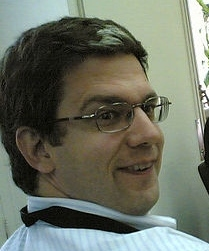
\includegraphics[width = 27
mm]{FTricas1.jpg},]
		\noindent \emph{Fernando Tricas García} es profesor
		titular de Lenguajes y Sistemas Informáticos del Departamento
		de Informática e Ingeniería de Sistemas de la Universidad de
		Zaragoza.  Empezó a estudiar la blogosfera casi cuando aún no
		existía (allá por el año 2002) y a tratar de integrarla en los
		cursos y tareas docentes un poco después.  Ha impartido
		numerosas charlas relacionadas con el tema de la Web 2.0, 
		internet y universidad,\ldots\ 
		Es actualmente Vicerrector de Tecnologías de la Información y
de la Comunicación.   
		\end{window}}}
%-------------------------------------------------

\noindent este sentido, esa realimentación debería ser, idealmente,
tan próxima a la prueba como sea posible.  El estudiante, por su
parte, debería tratar de obtener tanta información como sea posible,
bien de la corrección en sí misma, bien de su análisis posterior.

Y ya que estamos hablando de la enseñanza de la informática, habría
que hacer bastante énfasis en la palabra {\em práctica}.  Es evidente
que un ingeniero de caminos no va a poder construir los estribos de un
puente ferroviario durante un examen.  Tampoco en nuestros temas será
posible construir un sistema grande y complejo, pero en informática
tenemos a nuestra disposición todas las herramientas para evaluar en
la práctica si se ha aprendido o no un contenido que, esencialmente,
también es práctico.  Si un examen {\em teórico} de una asignatura
práctica puede ser discutible, más discutible aún es un examen {\em
escrito} de las {\em prácticas} de esa asignatura, algo
desgraciadamente bastante común todavía.  Sin olvidar que el acto de
la evaluación puede ser tan formativo como el propio trabajo, su
presentación, análisis y la interacción en torno a las cuestiones más
interesantes de la prueba, que pueden ayudar a determinar si realmente
se han adquirido los conocimientos, pero también pueden servir para
afianzarlos, reforzarlos y complementarlos.

Y de hecho, siendo la evaluación un acto de aprendizaje, cuanto más se
acerque a este formato, más precisa va a ser y más va a redundar en la
adquisición de conocimientos, de forma autónoma, por el
estudiante. Cierto es que las clases teóricas tienen una cantidad de
personas que impiden en la práctica la enseñanza personalizada, pero
también es cierto que las clases prácticas tienen un tamaño manejable
y que todas las plataformas de enseñanza hoy en día nos proveen de
todo tipo de herramientas para hacer un seguimiento personalizado, si
no personal, de los alumnos. 

Y esta es la última columna del último \ReVision; pero no debería ser
el final de la innovación en la enseñanza de la informática igual que
la evaluación no debe ser el final del proceso de aprendizaje.  Se
debe aprender siempre y, sobre todo, se debe de enseñar aprendiendo y
de aprender enseñando.  Esperamos haber aprobado la evaluación y,
quién sabe, si poder seguir escribiendo sobre estos temas en otro
contexto.  Han sido 22 columnas (contando esta) en las que hemos
tratado de interactuar entre los autores (con éxito, al menos en la
producción de las propias columnas) y con otras personas (con poco
éxito, a la luz de la falta de interacción y propuestas recibidas).

\smallskip

\noindent ¡Hasta pronto!

\medskip

\noindent\emph{Todas las columnas de la serie Docencia 2.0
pueden descargarse en formato LaTeX desde
\surl{https://github.com/ReVision-Docencia-20/Columnas}}

\noindent\rule{90mm}{1pt}

{\small \noindent
\includegraphics[height = 4ex]{CC.png} 2018 JJ.
Merelo, F. Tricas. Este artículo es de acceso libre distribuido bajo
los términos
de la Licencia Creative Commons de Atribución, que permite copiar,
distribuir y comunicar públicamente la obra en cualquier medio, sólido
o electrónico, siempre que se acrediten a los autores y fuentes
originales}

\end{multicols}
\end{document}

